%!TEX root = ../dokumentation.tex

\chapter{Mongo DB (Document)} \label{ch:mongo}
\chapterauthor{Linus Krebes, Fabian Mujdrica, Mika Santoro, and Tom Dankel}

\section{Type of Database \& History}
MongoDB was developed in 2007 by a New York-based organization 10gen which is now called MongoDB Inc. MongoDB was developed as a \ac{PAAS} initially.

Due to the need or idea of the database processing data in large amounts, according to Dwight, the database was named MongoDB, a word obtained from the term \enquote{humongous} \parencite{mongodb-History}.
Nowadays MongoDB is the most popular Document-oriented Database in use and the fifth most popular database management system worldwide \parencite{mongodb-Statista}.

Document-oriented databases, also known as document stores, are a type of NoSQL database that stores data as documents. Each document has a unique key and serves as the value in a key-value store. The main difference between key-value and document stores is that the latter contains metadata that provides structure to the data \parencite{mongodb-Comparison}.

Document databases typically have an \ac{API} or query language that allows developers to execute the \ac{CRUD} operations \parencite{mongodb-mongo}.

\begin{itemize}
    \item \textbf{Create:} Documents can be created in the database. Each document has a unique identifier.
    \item \textbf{Read:} Documents can be read from the database. The \ac{API} or query language allows developers to query for documents using their unique identifiers or field values. Indexes can be added to the database in order to increase read performance.
    \item \textbf{Update:} Existing documents can be updated — either in whole or in part.
    \item \textbf{Delete:} Documents can be deleted from the database.
\end{itemize}

Document-oriented databases allow for complex data structures, with the ability to nest documents within other documents. Unlike relational databases that spread object information across multiple tables, document stores can store all data for an object in a single document. These databases typically store data as \ac{JSON}, \ac{BSON}, \ac{XML}, or \ac{YAML} documents and can use \ac{SQL}, full-text search, or a native query language for data retrieval. Document stores are popular in e-commerce, blogging, analytics, and content management systems due to their flexible schema and scalability. Sharding is a common horizontal scaling strategy used to scale document stores, which are useful for storing large amounts of unrelated, complex information with varying structures \parencite{mongodb-Comparison}.

\begin{figure}[H]
    \centering
    \caption[Document Database vs SQL based Database]{Document Database vs SQL based Database \parencite{mogngodb-image}} \label{fig:Software pricing Overview}
    \includegraphics[width=1.0\textwidth]{images/Document_Database.png}
\end{figure}

\section{Differences Document Databases vs Relational Databases}

\textbf{The intuitiveness of the data model:} Working with documents is much more intuitive since they correspond to objects in code. Unlike with relational databases, there is no need to split data across tables, perform complex joins, or use a separate \ac{ORM} layer. Instead, data that is typically accessed together is stored together, resulting in less code for developers and improved performance for end users \parencite{mongodb-mongo}.

\textbf{The ubiquity of JSON documents:} The use of \ac{JSON} as a standard for data exchange and storage is now widely accepted. \ac{JSON} documents are lightweight, easy to read by humans, and don't rely on any specific programming language. These documents can represent any type of data model, allowing developers to structure data in the format that best suits their application, whether that's rich objects, key-value pairs, tables, geospatial and time-series data, or graphs consisting of nodes and edges \parencite{mongodb-mongo}.

\textbf{The flexibility of the schema:} Document schemas in document databases are both dynamic and self-describing, which eliminates the need for developers to predefine them in the database. As a result, the structure of fields in documents may differ from one document to the next. Developers are also free to modify the structure at any time, avoiding any disruptions caused by schema migrations. Certain document-oriented databases come equipped with schema validation, which allows developers to enforce rules related to document structures if they so choose \parencite{mongodb-mongo}.

\section{Database Design}

MongoDB belongs to the NoSQL database subcategory. The administration of a vast volume of data is one of the main reasons for its establishment. A document is used to handle the data, and it has a number of fields. Every document can have a significantly different length from the others \parencite{mungekar_2019}. There is no specified schema to produce or develop such documents, hence their structure totally depends on how the developers program it to be \parencite{taylor_2020}.
Ad hoc queries, indexing, workload balancing, and replication are all supported.
Always take the requirements of the application into account when modelling the data. After that, be certain to take the type of document into account. To get the most out of heavy data that needs to be modelled, indexing the data is always necessary. Also, it's important to regularly check on the CRUD operations. Use the sharding feature to boost efficiency if there are any irregularities \parencite{taylor_2020, mungekar_2019}.
In addition to this, MongoDB has a number of helpful clients and drivers for most of the popular programming languages.

In the following, the key components of MongoDB are further described.

\subsubsection{Database}

Similar to how RDMS uses containers for tables, this one is for collections. On the file system, every database receives a unique collection of files. Several databases can be stored on a MongoDB server \parencite{taylor_2020}.

\subsubsection{Collection}

A collection is a group of database documents. A table is what a collection would look like in an \ac{RDBMS}. One database contains the full collection. Regarding collections, there are no schemas. Although different documents contained inside a collection may have different fields, most documents in a collection are intended to serve the same function or to achieve the same end result \parencite{intellipaat_2016}.

\subsubsection{Document}

A group of key-value pairs can be referred to as a document. Dynamic schemas are linked to documents. A document in a single collection does not need to have the same structure or fields, which is a benefit of dynamic schemas. A collection document's common fields can also contain a variety of data types \parencite{intellipaat_2016}.

\subsubsection{Field}

A document's name-value pair. Documents can have zero fields or more. The equivalent of columns in relational databases are fields.

\subsubsection{Replication}

Replication is a crucial feature that protects against failures, increases data availability, and prevents data loss from one server.
Replica sets are the basis for MongoDB's replication. A collection of mongod instances hosting the same data set is known as a replica set. The primary or main node is chosen out of all nodes. The primary node is that one. The term "secondary node" refers to all others. To preserve consistency, the primary node receives all operations from the user, and the secondary nodes are updated from the primary one using the same operation. In the event that the primary node fails, one of the secondary nodes is chosen to serve as the primary node, and the operations continue. When the downed node recovers, it becomes one of the secondary nodes in the cluster. Mongo Atlas allows us to manage our cluster of Mongo instances. The concept of horizontal scalability and instance addition is the foundation for the creation of Mongo clusters \parencite{roy_databases_2020}.

\begin{figure}[H]
    \centering
    \caption[Replica set schematic]{Replica set schematic (inspired by \textcite{roy_databases_2020})} \label{fig:Replica Sets}
    \includegraphics[width=\textwidth]{images/Replica_Sets.jpeg}
\end{figure}

\subsubsection{Sharding}

MongoDB uses sharding to store data across several machines. In order to spread data and operations in response to the expansion of load and demand, it employs horizontal scaling to add more computers \parencite{roy_databases_2020}.

Sharding in MongoDB has 3 main components:

\begin{itemize}
    \item \textbf{Shards or replica sets:} Every shard functions as a different replica set. All the info is kept there. They aim to improve the data's availability and consistency.
    \item \textbf{Configuration Servers:} They resemble the cluster managers. The metadata for the cluster is stored on these servers. Indeed, they already have the data from the cluster mapped to the shards. In order to target the appropriate shard when a query is received, query routers employ these mappings from the configuration servers.
    \item \textbf{Query Router:} Mongo entities that act as user application interfaces make up the query router. They receive user requests from the applications and provide the necessary answers to the applications. Typically, each cluster has numerous query routers to distribute load.
\end{itemize}

\begin{figure}[H]
    \centering
    \caption[Replica set schematic]{Replica set schematic (inspired by \textcite{mongodb_sharding})} \label{fig:Sharding}
    \includegraphics[width=\textwidth]{images/sharding.jpeg}
\end{figure}

\section{Installation}

MongoDB offers various implementation options, including local installation and server deployment. The advantages of using a local MongoDB include increased flexibility and control. However, the responsibility for maintenance and system security lies with the user, as it is hosted on their own server. \parencite{mujdrica_whatismongodb}

In addition, MongoDB can be executed within a containerized environment to support secondary services. Containerization provides benefits such as rapid provisioning, scalability, and portability, making it a useful option for deploying MongoDB. \parencite{mujdrica_docker}

Moreover, MongoDB can be utilized as a Database as a Service (DBaaS), allowing developers to focus on their applications without managing the underlying infrastructure. Prominent examples of DBaaS providers include MongoDB Atlas and AWS. MongoDB as a DBaaS solution offers easy scalability, high availability, automated backups, and maintenance. These features make it a popular choice for organizations seeking to streamline their database management processes. \parencite{mujdrica_aws}

\subsubsection{Installation MongoDB Community Edition}

The MongoDB service includes two different versions: The Enterprise Edition and a free Community Edition. This example is based on the Community Edition, since it´s more affordable and easy to install. There are Installerpackages for all important operating systems, including Windows, Linux and MacOS. Furthermore the Community Edition can be integrated into a Docker-Container-Environment directly through the intended installer. To install MongoDB on a windows operating system, there´s foremost the need of a 64-Bit Version of windows itself. The minimal requirements include atleast 4GB of free memorystorage and 1 GB \ac{RAM}, nevertheless there´s a recommendation to use atleast 4 GB of \ac{RAM} to make the program run more smoothly. Through the installer it´s possible to directly install important tools and widgets to support your work. Using this feature, one can choose different drivers to support different coding languages. Additionally the so called MongoDB compass can be installed. This feature is a visual tool to aid in the management of the MongoDB instances. \parencite{mujdrica_community}

\section{API}

There exist several types of APIs that can be employed to access MongoDB, including terminals and \acp{CLI}. Terminals facilitate the creation, retrieval, and modification of databases, collections, and files. Additionally, scripts can be generated to automate repetitive processes. Furthermore, MongoDB provides a \ac{REST}ful \ac{API} that allows users to access and modify data via \ac{HTTP} requests. This provides a flexible alternative to traditional access methods.

\subsection{MongoDB Compass}

MongoDB Compass is an application designed to manage specific MongoDB instances. It provides all of the features of terminal access, while also offering a user-friendly graphical interface to streamline database management \parencite{mujdrica_compass}.

\begin{figure}[H]
    \centering
    \caption{MongoDB Compass user interface} \label{fig:compass}
    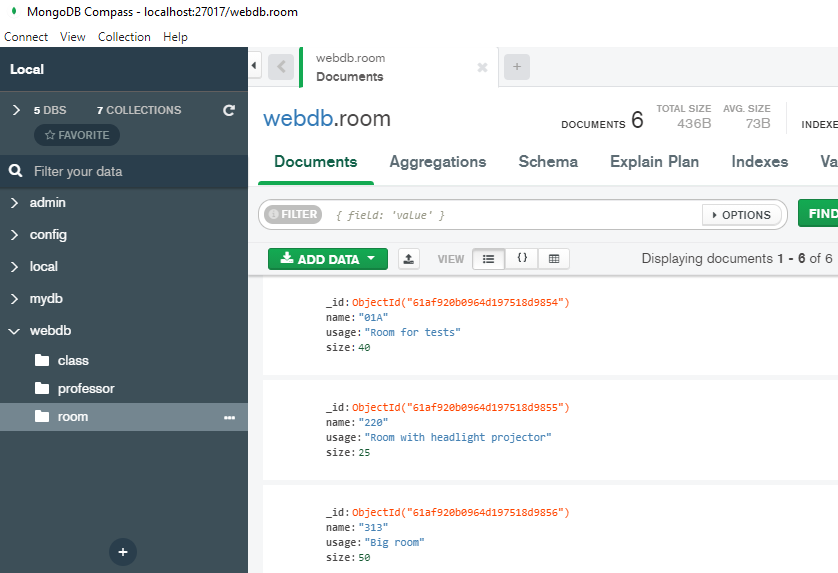
\includegraphics[width=1.0\textwidth]{images/mujdrica/compass.png}
\end{figure}

This image depicts the user interface of MongoDB Compass. Upon inspection of the topmost uniform resource locator (URL), it becomes apparent that the application has established a connection with the database through the default port. On the left side, a comprehensive list of accessible databases is available. Specifically, the showcased collection is labeled as 'room' and is associated with the 'webdb' database. Additionally, each record features unique identifiers as well as corresponding attributes such as 'name', 'usage', and 'size'. Notably, the application provides various sorting configurations to facilitate the filtering of files based on specific values. MongoDB has other useful features, such as creating schemas.

\subsection{Drivers}

Official MongoDB drivers are available for all common used programming languages, including Python, Java, C++ and other programming languages. These drivers enable direct connections to the MongoDB database service \parencite{mujdrica_drivers}.

\subsubsection{Example}

The following example shows how to use the library pymongo to access a MongoDB database in Python.  The following command in a CLI can be used to install the library \parencite{mujdrica_pymongo}.

\begin{verbatim}
pip install pymongo
\end{verbatim}

Now the database can be accessed. First, a connection to the database is established. Then a collection can be opened and read out.

\begin{verbatim}
import pymongo

client = pymongo.MongoClient('localhost', 27017)
db = client['webdb']
collection = db['class']

first_entry = collection.find_one()
print('ID: ', first_entry['id'])
print('Name: ', first_entry['name'])
\end{verbatim}

\section{Comparison MongoDB/MySQL}

Now a MySQL database is to be mocked up with MongoDB. Afterwards, both types of database will be compared with each other based on various criteria. The existing MySQL database has the following schema.

\begin{figure}[H]
    \centering
    \caption{Schema of the sample MySQL database} \label{fig:mysql_schema}
    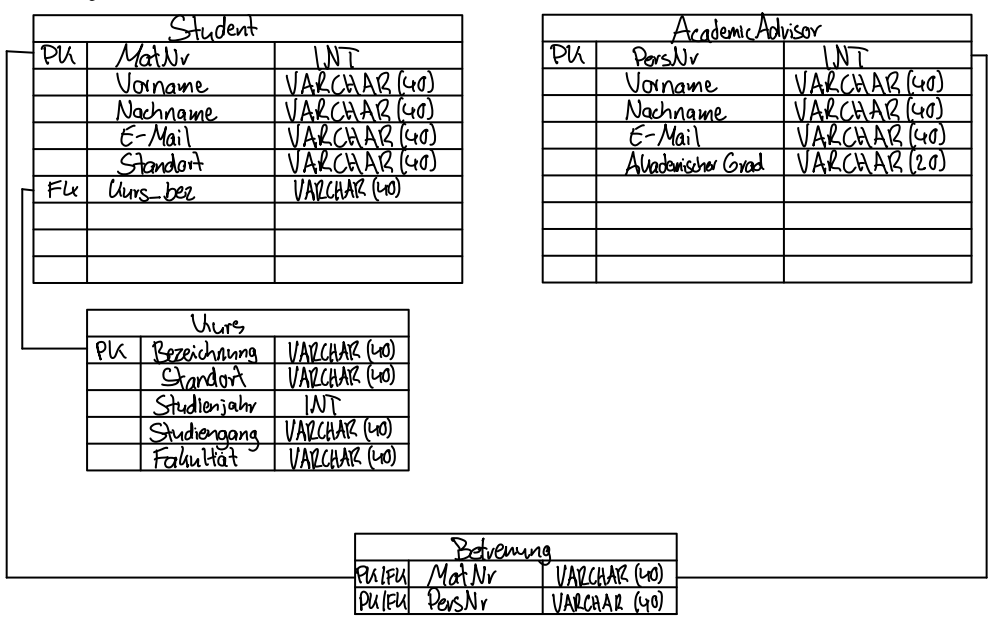
\includegraphics[width=1.0\textwidth]{images/mujdrica/mysql_schema.png}
\end{figure}

\subsection{Replication with MongoDb}

To replicate the database in MongoDB, each table is first created as a collection. The following code creates the collections using Python \parencite{mujdrica_pymongo}.

\begin{verbatim}
import pymongo

client = pymongo.MongoClient("mongodb://localhost:27017/")
db = client["replication"]

# Create Collections
students_col = db["students"]
courses_col = db["courses"]
academic_advisors_col = db["academic_advisors"]
supervision_col = db["supervision"]
\end{verbatim}

Afterwards, the data can now be copied from the MySQL database to the MongoDB database. For the table 'Student' the code can look like this \parencite{mujdrica_mysqldriver}.

\begin{verbatim}
import pymysql

mysql_conn = pymysql.connect(
    host="localhost",
    user="username",
    password="password",
    database="testdb"
)

# Call Data from table 'Student'
mysql_cursor = mysql_conn.cursor()
mysql_cursor.execute("SELECT * FROM Student")
students_data = mysql_cursor.fetchall()

#insert data into the mongodb database
for student in students_data:
    student_doc = {
        "matNR": student[0],
        "vorname": student[1],
        "nachname": student[2],
        "email": student[3],
        "standort": student[4],
        "kurs_bez": student[5]
    }
    students_col.insert_one(student_doc)
\end{verbatim}

\subsubsection{Data query}

When performing a query between multiple tables in MySQL, joins are used. The following query returns all students that are hosted by an AcademicAdvisor with id 1.

\begin{verbatim}
SELECT s.* FROM Student s
INNER JOIN Betreuung b ON s.matNR = b.FK_MatNR
INNER JOIN AcademicAdvisor a ON b.FK_persNR = a.persNR
WHERE a.PersNr = 1;
\end{verbatim}

If you want to read the same information from the MongoDB database, you cannot simply use joins. Instead, a query can be performed as follows \parencite{mujdrica_joinsupdate}.

\begin{verbatim}
students_col = db["students"]
supervision_col = db["supervision"]
advisors_col = db["academic_advisors"]

#find academic advisor with id 1
advisor = advisors_col.find_one({"PersNR": 1})

students = supervision_col.find({"FK_persNR": advisor["_id"]}, 
    {"FK_MatNR": 1})
matnrs = [s["FK_MatNR"] for s in students]

result = students_col.find({
    "$and": [
        {"kurs_bez": {"$ne": None}},
        {"matNR": {"$in": muller_matnrs}}
    ]
})

for student in result:
    print(student)
\end{verbatim}

\subsection{Comparison}

MongoDB is a \ac{NoSQL} database system that does not rely on chart relationships, as is the case with relational databases such as MySQL. As a result, there are some differences in the way data can be modeled in MongoDB compared to relational databases.

In MongoDB, each document is assigned a unique id field by default, which serves as the primary key. This field is generated automatically during document creation but can also be set manually. Unlike relational databases, MongoDB does not employ foreign keys as there are no table relationships. Instead, a document's id field can be stored as a reference in another collection to refer to data in one document \parencite{mujdrica_comparison}.

MongoDB does not support traditional joins, instead retrieving data by embedding or referencing documents in other collections. Embedding entails storing a document within another document, while referencing involves storing a reference to another document. MongoDB supports a kind of joins since version 3.2 \parencite{mujdrica_comparison, mujdrica_joinsupdate}.

Unlike relational databases, where a schema is established before data insertion, MongoDB does not have set rules for a schema as each record can be individual. Nevertheless, MongoDB supports a flexible schema, allowing fields to be added or removed from a document without changing the schema \parencite{mujdrica_comparison}.

MongoDB provides functions similar to relational databases for aggregating data, such as GROUP BY, COUNT, AVG, MAX, MIN, and others, but there are syntax and usage differences \parencite{mujdrica_comparison}.

It is crucial to note that MongoDB does not support cascading, a common feature in relational databases. If a document that references data in other collections needs to be deleted, a manual command or a script must be used in the MongoDB environment to accomplish it. As a result, modeling data in MongoDB varies from relational databases, with certain aspects, such as defining a primary key, being simpler to implement, while others, such as joins, necessitating a more extended process of embedding or referencing data. However, the best approach for modeling data in MongoDB varies depending on the application's specific requirements \parencite{mujdrica_comparison}.

\section{Advantages and Disadvantages}

\subsection{Advantages}

\textbf{Flexible data model}: MongoDB uses a flexible document data model that allows you to store data in a variety of ways. This makes it easy to adapt to changing business needs and to scale your data as your application grows \parencite{mongodb-datamodels, knowledgenile-pro-con}. 

\textbf{High scalability}: MongoDB is designed to handle large amounts of data and high traffic loads. With sharding it can be easily scaled horizontally by adding more nodes to a cluster \parencite{mongodb-scalability, dataflair_2018}. Furthermore, replica sets enable high availability, handling of redundancy/failover, and less read operation bottlenecks \parencite{mongodb-replica-sets}.

\textbf{High performance}: MongoDB uses a number of performance optimizations such as memory-mapped files, asynchronous I/O, and indexing to provide high throughput and low latency \parencite{mongodb-performance, knowledgenile-pro-con}.

\textbf{Rich query language}: MongoDB provides a powerful query language that supports a variety of operators and expressions for filtering, sorting, and aggregating data \parencite{mongodb-query}.

\textbf{Easy Environment and Setup}: MongoDB requires little setup time and minimal effort to use. Modern JavaScript frameworks are available, and it is quicker and simpler to set up than \ac{RDBMS}.
Because of this functionality, users can choose NoSQL architectures with confidence. In addition, compared to SQL databases, it offers faster options for learning and training \parencite{knowledgenile-pro-con, jamsheer_2019}.

\subsection{Disadvantages}

\textbf{Limited Data Size}: MongoDB only permits documents with a maximum size of 16 MB per default. For files larger than 16 MB they refer to the GridFS \ac{API} \parencite{mongodb-documents}.

\textbf{No schema enforcement}: MongoDB does not enforce a strict schema, which can lead to data inconsistencies if the data is not carefully structured and validated.

\textbf{Higher memory usage}: MongoDB needs a lot of storage since it lacks join functionality, which causes data duplication. The amount of redundant data keeps increasing, which requires extra memory space \parencite{knowledgenile-pro-con}.

\textbf{Complexity}: MongoDB's flexible data model and lack of strict schema enforcement can make it more complex to design and manage compared to traditional databases. It may also require more expertise to optimize performance and scale effectively.

\section{MongoDB and the CAP-Theorem}

\subsection{CAP-Theorem}

The \ac{CAP}-Theorem was proofed by Gilbert and Lynch in 2002 \parencite{brewer:2002}. They published an axiomatic indirect proof of Brewers conjecture. Eric Brewer presented his conjecture in a \ac{PODC} talk at the University of Carolina in 2000 \parencite{brewer2000towards}. The \ac{CAP}-Theorem states that it is not possible to guarantee consistency, availability and partition tolerance simultaneously in a distributed system. It is only possible to satisfy two of these properties simultaneously \parencite[1]{brewer:2002}.

\subsubsection*{Consistency}

To meet this criterion, the distributed system must ensure consistency of data after a completed transaction. Therefore, in a distributed system with replicated data, all replicated data must be updated after a transaction is completed. This way, all nodes have the same data at any point in time \parencite[2\psqq]{brewer:2002}.

\subsubsection*{Availability}

Availability of a distributed system means that all requests received by a non-failing node in the system gets a response. It means in combination with the need for partition tolerance that every request must terminate, even with the occurrence of severe network failures \parencite[3]{brewer:2002}.

\subsubsection*{Partition Tolerance}

A partition tolerant network may only react incorrectly in the event of a total failure of the network. Therefore, the network may lose any number of messages between nodes and must still function correctly. All messages between two nodes in two different components are lost when the network is partitioned. \parencite[3\psqq]{brewer:2002}.

\subsection{Proof}

Assume a consistent, available and partition tolerant algorithm executed in a partitioned distributed system with a value v$_{0}$. Due to the message loss, a write with v$_{1}$ on v$_{0}$ in one partition is not recognized in the other partition. A read in the other partition on the variable will return v$_{0}$. This contradicts the Consistency property, because the return must be v$_{1}$, not v$_{0}$. Due to availability and partition tolerance the network must respond although the message loss. The contradiction above proofs that no distributed system can guarantee consistency, availability and partition tolerance \parencite[4\psqq]{brewer:2002}.

\subsection*{Consistency vs. Availability (vs. Partition Tolerance)}

The \ac{CAP}-Theorem refers to distributed systems. For these, choosing between two properties that do not include partition tolerance does not make sense. In this case, the \ac{CAP}-Theorem means choosing between consistency of data or availability of the system.

\subsubsection*{Consistency and Partition Tolerance}

A consistent and partition tolerant network responds to partitions by losing availability. The nodes that are unreachable and therefore not guaranteed to be consistent are simply unavailable until connectivity is reenabled and consistency is guaranteed to be restored \parencite[6]{brewer:2002}.

\subsubsection*{Availability and Partition Tolerance}

An available and partition tolerant network responds to a partition with loss of consistency. All nodes remain available, but the response is not necessarily consistent. Responses are consistent again after connectivity is restored \parencite[6]{brewer:2002}.

\subsection*{Position of MongoDB in CAP}

MongoDB is a \ac{CP} tolerant database. MongoDB chooses consistency over availability if a partition occurs. The replica sets are responsible for this behavior \parencite{stackoverflow:2023}.
The primary node of a replica set is the only node that accepts write requests. Normally, read requests are also directed to the primary node. A network partition detaches any number of nodes. The disconnected nodes can no longer communicate with the remaining nodes. A new primary node is elected only if the primary node can reach only a minority of nodes because the primary node is not in the majority. The election of a new primary node takes a few seconds. This process makes the system unavailable for write and read requests for a short time to ensure consistency.

Increasing the availability of the system is possible only if the strong consistency is broken. In read preference mode, it is allowed to read from secondary nodes. The primary node is still the only node allowed to accept write requests. In case of partitioning, it is possible that the detached secondary nodes have stale data because the message with new data from the primary node has been lost.

To improve the weakened consistency, pass a write option. A write request is successful only if the primary node has received as many acknowledges as defined/acknowledges from at least half of the nodes. This is called eventual consistency (a tradeoff between consistency and availability). Despite the increased availability for read requests, writes are still not possible if the primary node is not available or is currently in the election phase. It should be noted that increased availability means decreased consistency (eventual consistency), and the focus remains on consistency and partition tolerance \parencite{katwal:2020}.